\documentclass[twoside]{article}
%\usepackage{graphicx}
%\usepackage{caption}
\usepackage{subcaption}
\usepackage[letterpaper, margin=1in]{geometry}
\usepackage{float}
\usepackage{fancyhdr}
\usepackage{tikz}
\usepackage[utf8]{inputenc}
\usepackage{ifthen}
\usepackage{tabu}
\usepackage[shortlabels]{enumitem}
\usepackage{amsmath}
\usetikzlibrary{fadings}



\pagestyle{fancy}
\fancyhead{}
\fancyhead[L]{\ifthenelse{\isodd{\value{page}}}{APS Logbook}{\textbf{\rightmark}}}
\fancyhead[R]{\ifthenelse{\isodd{\value{page}}}{\textbf{\rightmark}}{Election 2016}}
\renewcommand{\headrulewidth}{1pt}
\fancyfoot{}
\fancyfoot[L]{\ifthenelse{\isodd{\value{page}}}{}{Page \thepage}}
\fancyfoot[R]{\ifthenelse{\isodd{\value{page}}}{Page \thepage}{}}



\title{American Political Systems Logbook}
\author{Noah Stockwell}
\date{2016}

\begin{document}
\begin{titlepage}
  \centering
  \begin{tikzpicture}[overlay]
  \path (0,0) rectangle (\paperwidth,\paperheight);
  \node[scope fading=west,inner sep=0pt,outer sep=0pt,anchor=north east,opacity=0.3] at(20,3) {
\includegraphics[height=1.0625\paperheight]{images/frontpage/flag.jpg}};
  \end{tikzpicture}
  \centering
  \begin{figure}[H]
    \centering
    \begin{subfigure}{.4\textwidth}
      \centering
      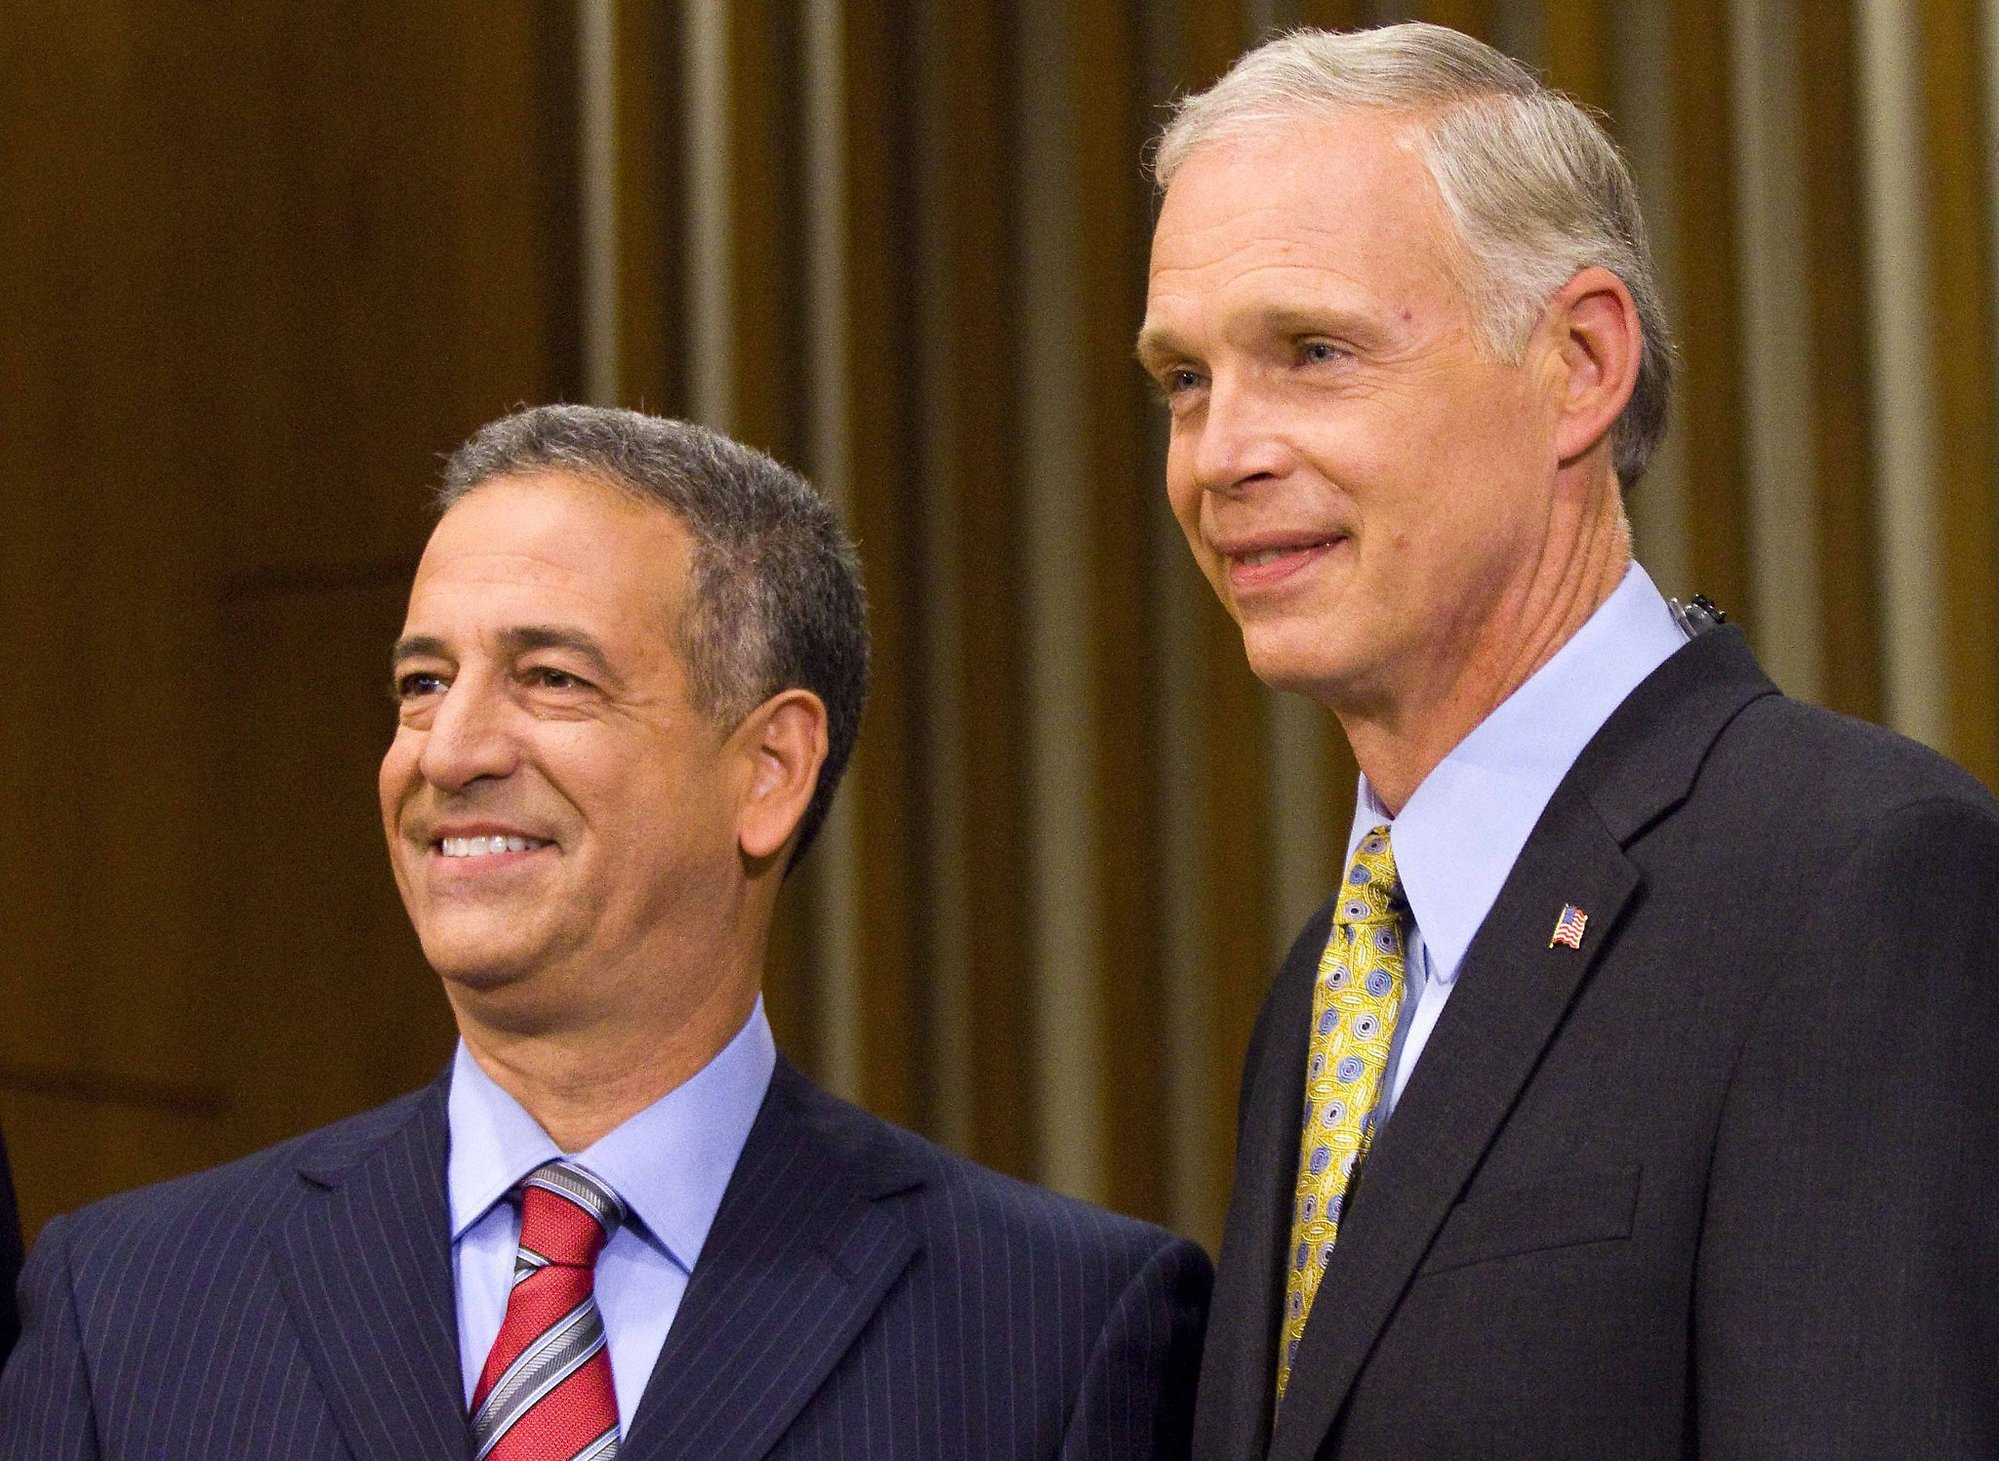
\includegraphics[width=6cm,height=4.5cm]{images/frontpage/Senate.jpg}
      \end{subfigure}%
      \begin{subfigure}{.4\textwidth}
        \centering
        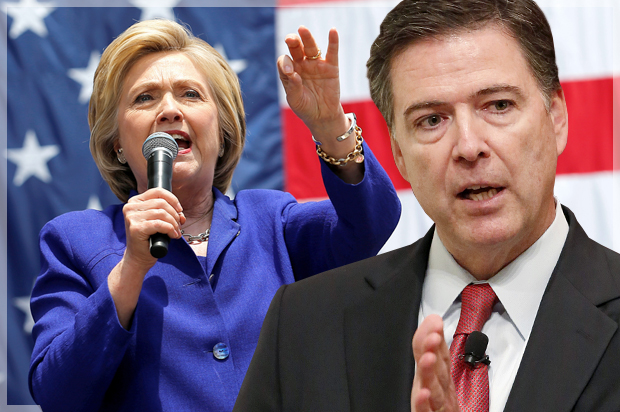
\includegraphics[width=6cm,height=4.5cm]{images/frontpage/Comey.jpg}
      \end{subfigure}%
      \centering
      \vskip3cm
    \end{figure}
    {\bfseries\huge American Political Systems Logbook\\}
    \vskip1cm
    {\bfseries\LARGE Election 2016\\}
    \vskip2cm
    {\huge Noah Stockwell\\}

    \centering
    \vskip2cm
    \centering
    \begin{figure}[H]
      \centering
      \begin{subfigure}{.4\textwidth}
        \centering
        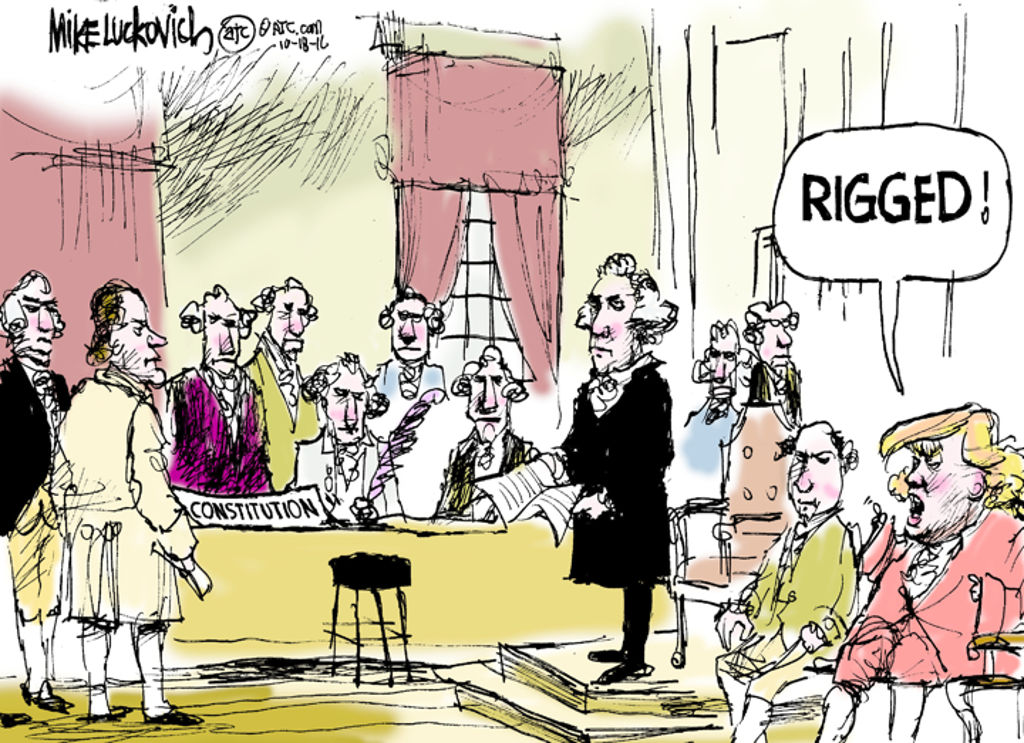
\includegraphics[width=6cm,height=4.5cm]{images/frontpage/Rigged.jpg}
        \end{subfigure}%
        \begin{subfigure}{.4\textwidth}
          \centering
          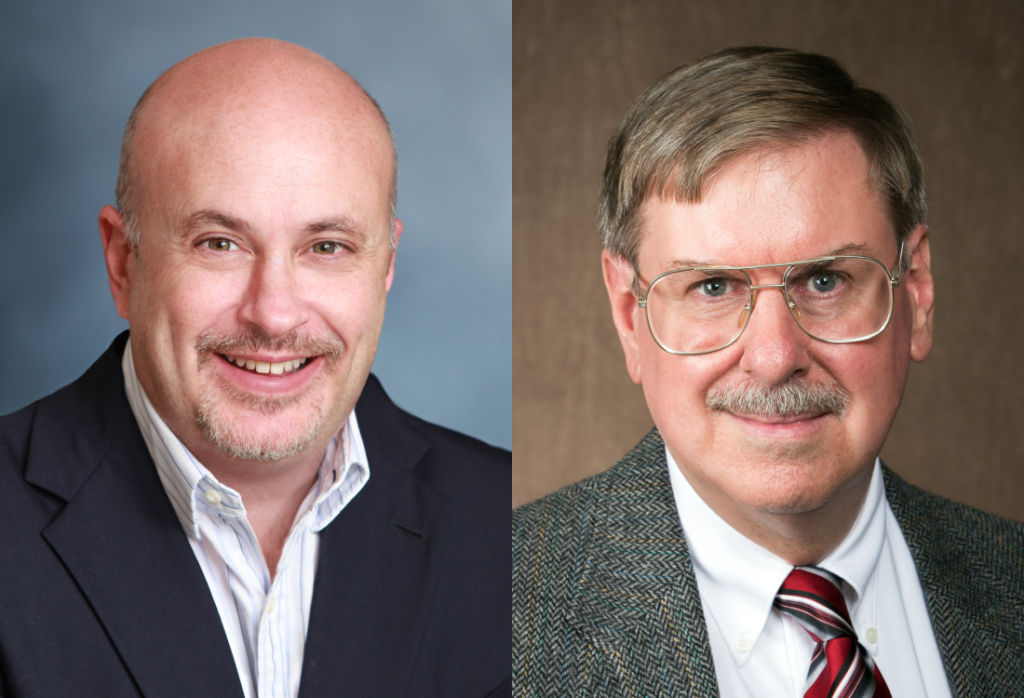
\includegraphics[width=6cm,height=4.5cm]{images/frontpage/House.jpg}
        \end{subfigure}%
      \end{figure}
\end{titlepage}
\tableofcontents
\newpage
\section{Candidate Bios}
\vskip1cm
\begin{center}
\begin{tabu} to 0.8\textwidth { X[c] X[c]}
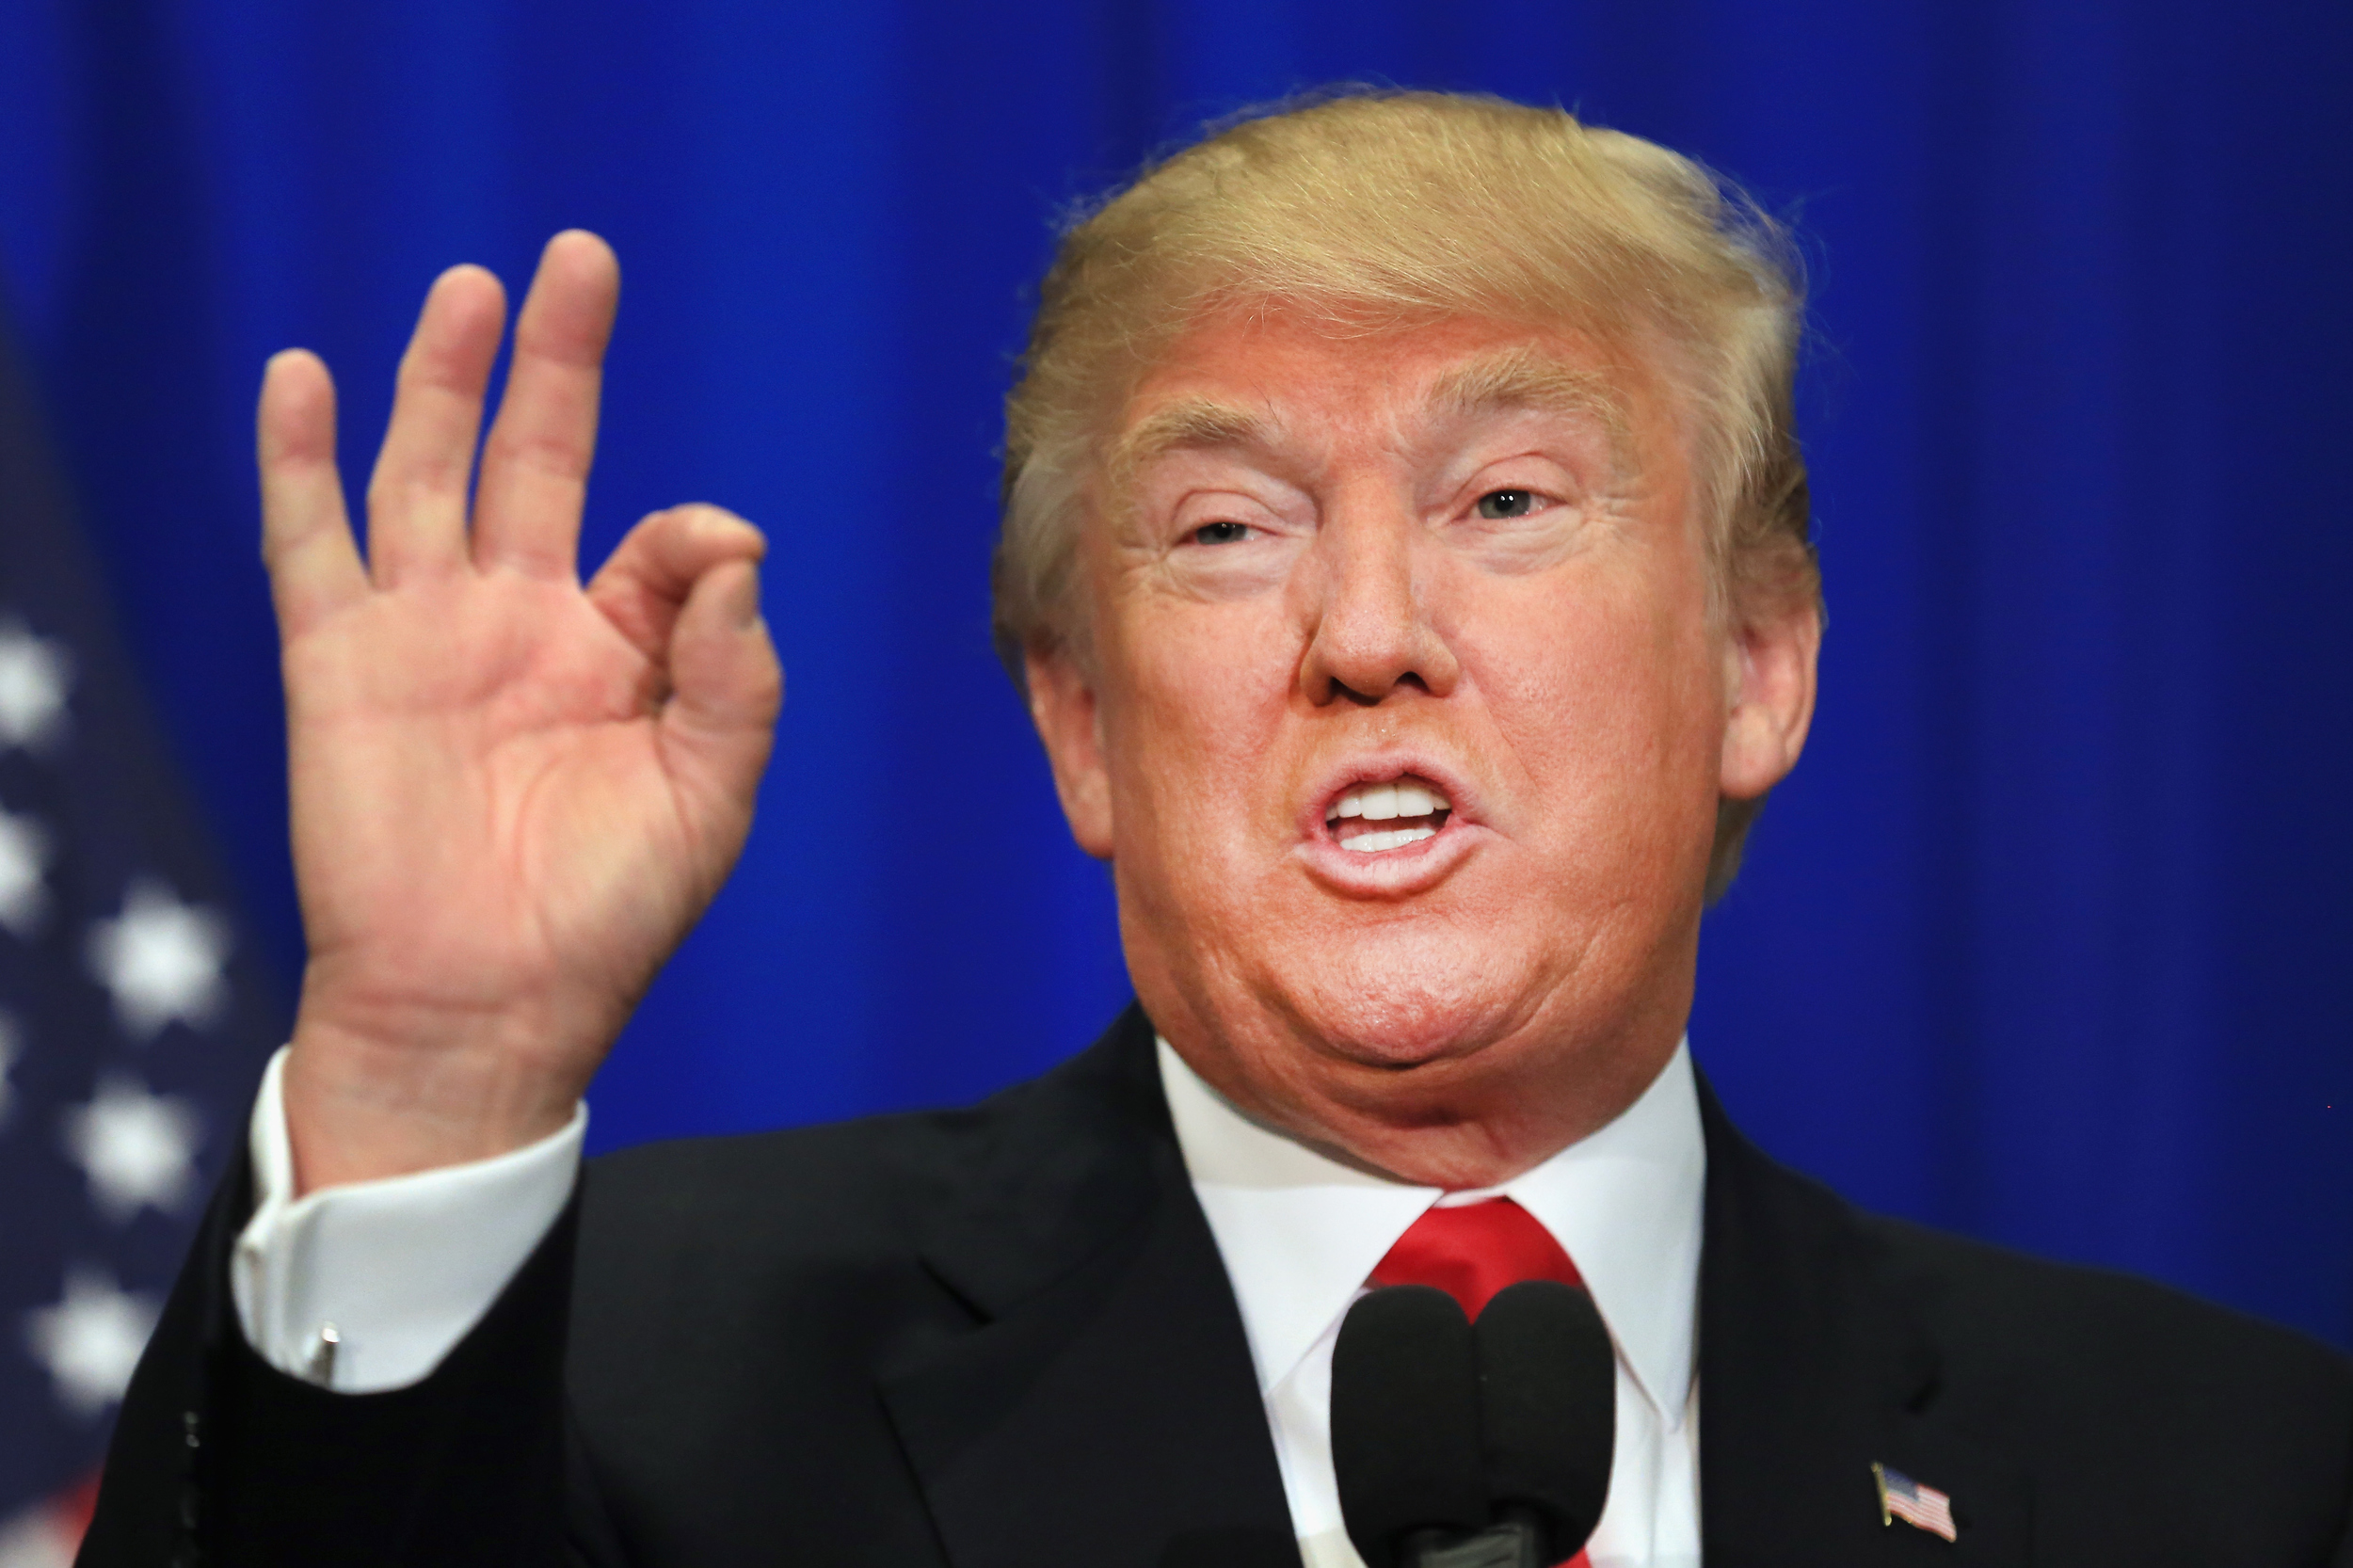
\includegraphics[width=6cm,height=4.5cm]{images/profiles/trump.jpg}
 \vskip0.5cm
 {\bfseries\Large Donald Trump}
 \begin{enumerate}[a)]
   \item Republican
   \item Bachelor's Degree in Economics from U-Penn
   \item None; he is a businessman
   \item Married and divorced, with kids
 \end{enumerate}
 &
 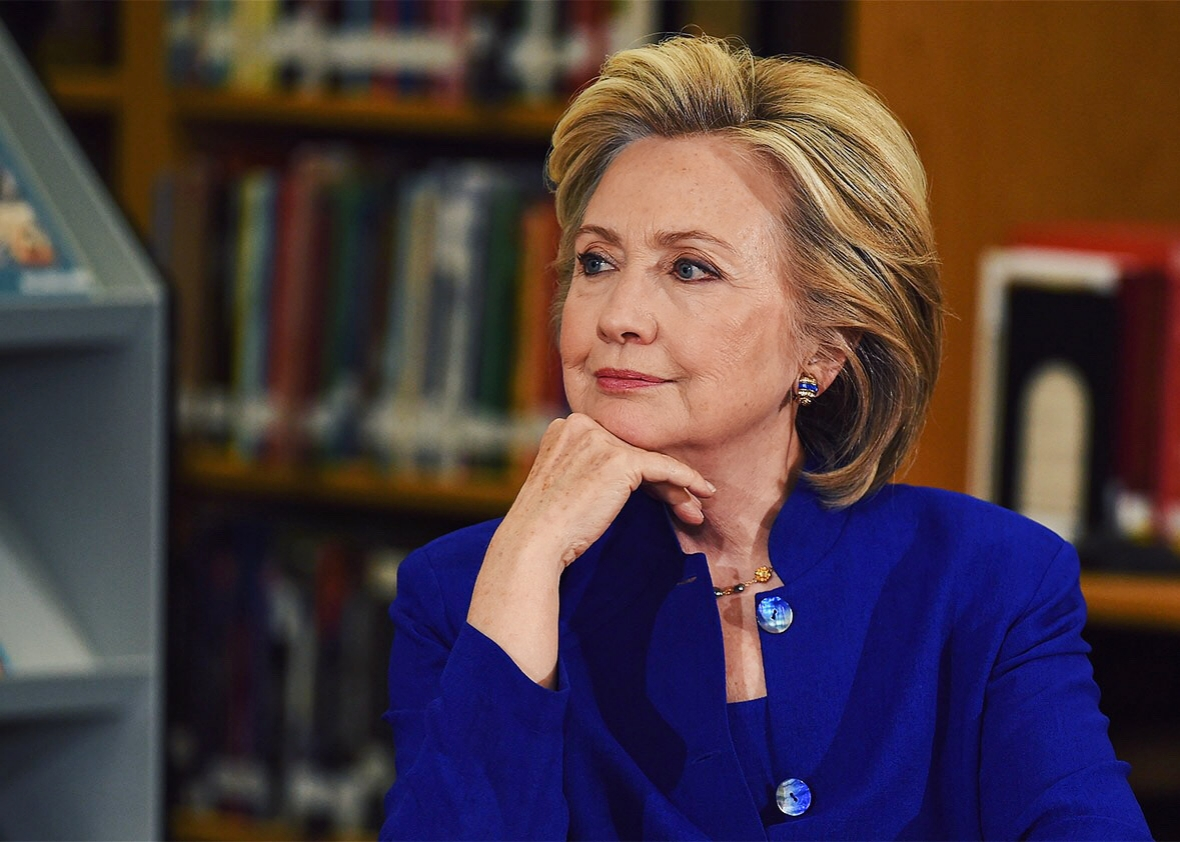
\includegraphics[width=6cm,height=4.5cm]{images/profiles/clinton.jpg}
  \vskip0.5cm
 {\bfseries\Large Hillary Clinton}
 \begin{enumerate}[a)]
   \item Democrat
   \item J.D. from Yale
   \item New York Senator, Secretary of State (not elected), First Lady
   \item Married, one daughter
 \end{enumerate}\\
 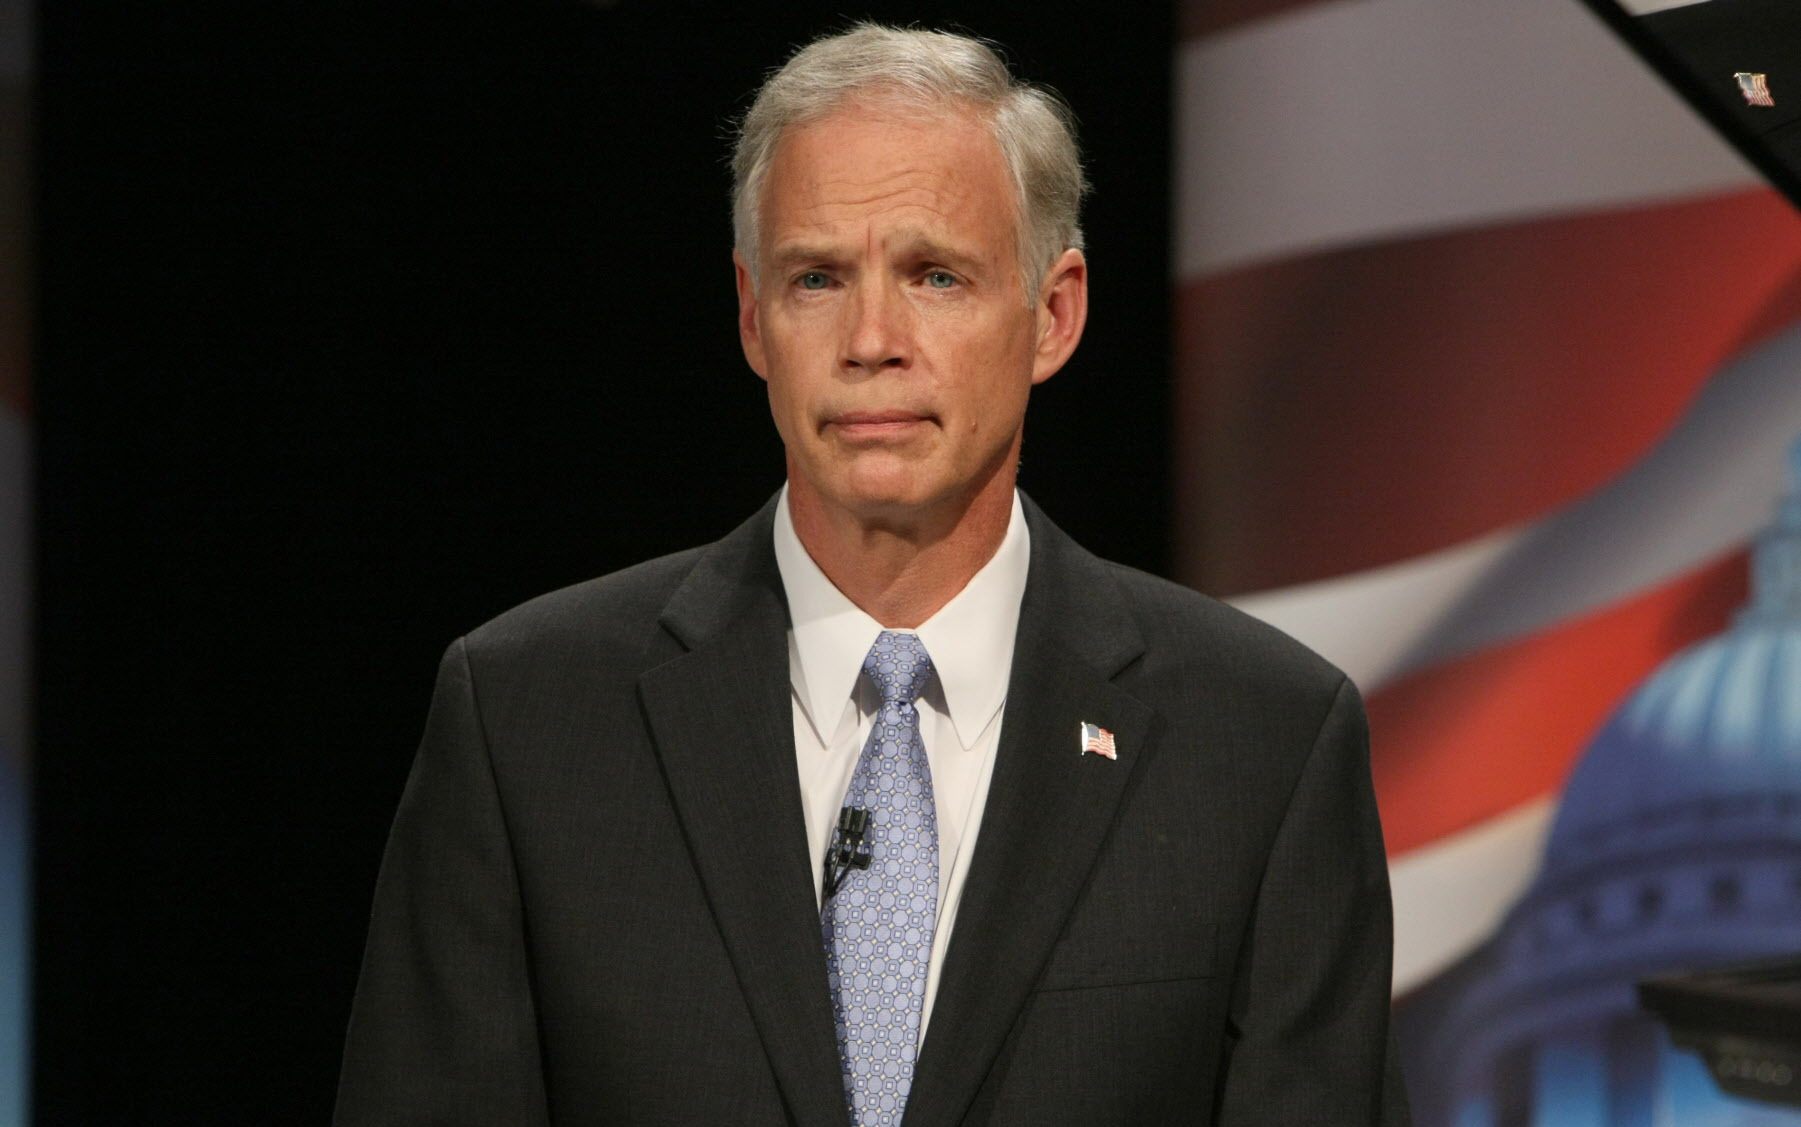
\includegraphics[width=6cm,height=4.5cm]{images/profiles/johnson.jpg}
 \vskip0.5cm
 {\bfseries\Large Ron Johnson}
 \begin{enumerate}[a)]
   \item Republican
   \item Bachelor's Degree in Economics from U-Penn
   \item None; he is a businessman
   \item Married and divorced, with kids
 \end{enumerate}
 &
 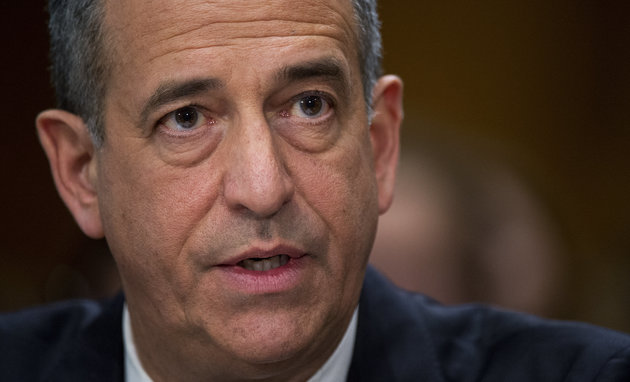
\includegraphics[width=6cm,height=4.5cm]{images/profiles/feingold.jpeg}
  \vskip0.5cm
 {\bfseries\Large Russ Feingold}
 \begin{enumerate}[a)]
   \item Democrat
   \item J.D. from Yale
   \item New York Senator, Secretary of State (not elected), First Lady
   \item Married, one daughter
 \end{enumerate}
 \end{tabu}
 \begin{tabu} to 0.8\textwidth { X[c] X[c]}
  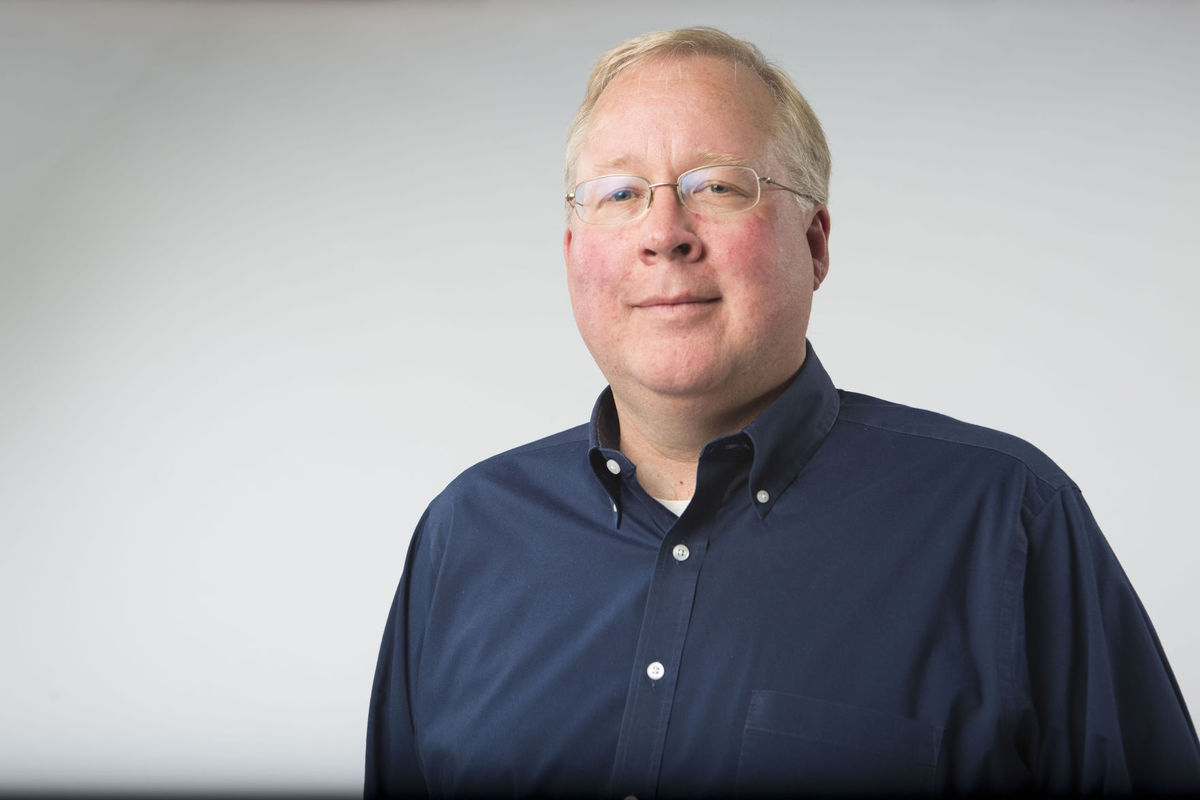
\includegraphics[width=6cm,height=4.5cm]{images/profiles/anderson.jpg}
 \vskip0.5cm
 {\bfseries\Large Phil Anderson}
 \begin{enumerate}[a)]
\item Libertarian
\item BA in Geography from UW-Madison and Applied Theology from Balamand
\item No experience
\item Married, two kids
 \end{enumerate}
 & \\
  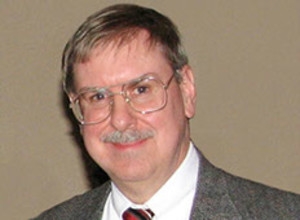
\includegraphics[width=6cm,height=4.5cm]{images/profiles/theron.jpg}
 \vskip0.5cm
 {\bfseries\Large Peter Theron}
 \begin{enumerate}[a)]
\item Republican
\item PhD from UW-Madison in mathematics
\item Instructor at Madison College
\item Married
 \end{enumerate}
 &
 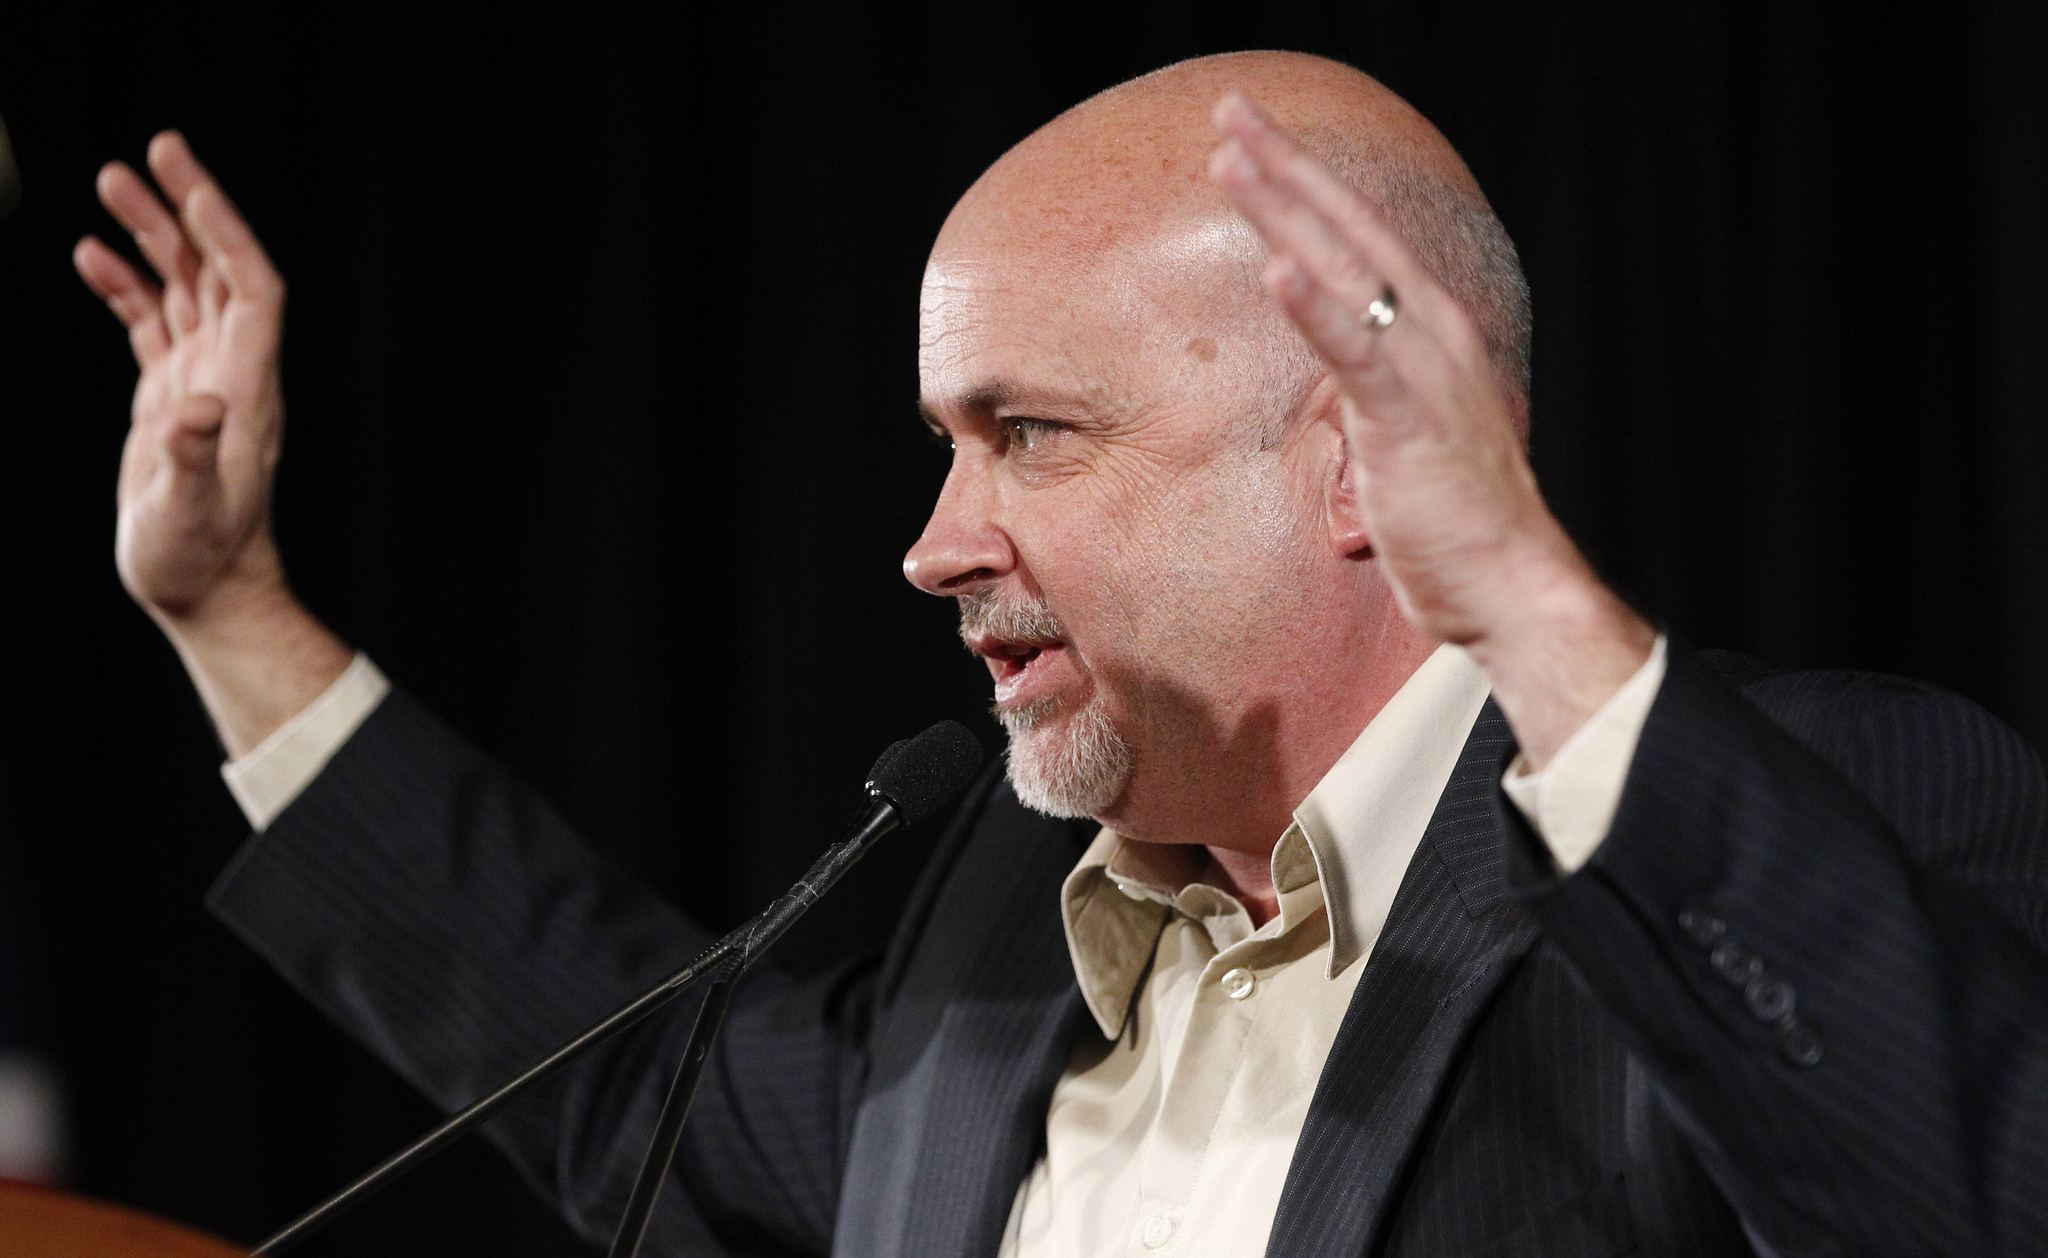
\includegraphics[width=6cm,height=4.5cm]{images/profiles/pocan.jpg}
  \vskip0.5cm
 {\bfseries\Large Mark Pocan}
 \begin{enumerate}[a)]
\item Democrat
\item Journalism Bachelor's from UW-Madison
\item Wisconsin Assembly, US House
\item Openly gay and married in Canada
 \end{enumerate}
\end{tabu}
\end{center}
\newpage
\section{Articles}
\subsection{September}
\centering
    \vskip2cm
    \begin{figure}[H]
      \centering
      \begin{subfigure}{.4\textwidth}
        \centering
        
\includegraphics[width=6cm,height=4.5cm]{images/articles/pepe0.jpg}
        \end{subfigure}%
        \begin{subfigure}{.4\textwidth}
          \centering
          
\includegraphics[width=6cm,height=4.5cm]{images/articles/pepe1.jpg}
        \end{subfigure}%
      \end{figure}
\paragraph{Pepe} Donald Trump is not a traditional republicans and does not have the the traditional republican base behind him. The ‘Alt-Right’ is a big part of his constituency - a newly formed group that resides strongly on 4Chan and r/The\_Donald on Reddit. They are the group that falls into what Hillary Clinton labeled the ‘Basket of Deplorables’. They participate in brigading, hacking, and their group has expanded to include Neo-Nazis and other hate groups. They, especially those on r/The\_Donald and 4Chan’s /pol, use an internet meme called Pepe. Pepe is an old comic that the original creator has disowned and recognized as a hate symbol. Many other groups have also officially recognized Pepe as a hate symbol, too. Donald Trump and his son, who has actively re-shared these comics of his father and Pepe, sometimes together, have both denied that this is white supremacy, but those who publicly identify as white supremacists, such as David Duke, have taken ownership of this cartoon.\\
Pepe was not originally a hate symbol and is not only a hate symbol today. It can be used with good intentions and without the purpose of white supremacy. That being said, it is close to the symbol of the Swastika. It was not originally a hate symbol and can be used as a symbol of divine power today, but its use has been hijacked by Nazis. Pepe and the Swastika are similar in that way, and when one sees Pepe today, there is a high probability that it is in fact supporting white supremacy.
\newpage
\subsection{October}
\subsubsection{October I}
\paragraph{Clinton's Speeches} Clinton has been the target of many hackers this election. In fact, Donald Trump is on record encouraging the Russians to hack her emails. He and his base rejoice whenever WikiLeaks releases another pile of information. This time, they have released transcripts of her speeches that she gave to the big banks on Wall Street. She later confirmed that this is is true: she said that it is important for a politician to have a public and private policy. She explained that it has been useful to some of the greats, such as Abraham Lincoln, who relied on white lies and deception to free the slaves.
\subsubsection{October II}
\paragraph{The Third Presidential Debate} Donald Trump cannot keep his mouth shut for the life of him. He has had no qualms about interrupting Hillary in debates, starting in the first debate. He interjected “wrong” and other words when Hillary was trying to speak. In the last debate, Trump interrupted and took Clinton’s bait when she called him a puppet of Russia. When she was talking about him and trying to bait him again, he leans into the microphone and says, “Such a nasty woman”. The live audience audibly gasped. This just gives Clinton’s claim that he doesn’t respect women more evidence, and he is unable to realize that he is only hurting himself.
\newpage
\subsection{November}
\paragraph{Email Conclusion} The FBI has finished going through emails from Clinton that they obtained from former Representative Anthony Weiner’s devices. It turns out that they already had all of the emails and the ones that they didn’t were personal. Donald Trump and his supporters are outraged, although more mainstream Republicans have already seen the records and agree that no charges could be brought against her. She has been tried many times by Republicans seeking to remove her from power. She has been cleared of any wrongdoing in the Benghazi mess eight times, and now twice for her emails. The chants of lock her up are misinformed, as much of this election has been. Recently, SNL’s Alec Baldwin said (of Trump about the truth), “[The truth] doesn’t matter. I’ve said it and now half the country believes it.”
\newpage
\section{Fourier Analysis}
\vskip4cm
\paragraph{Why Fourier?} Fourier allows us to generate a function of sines and cosines to approximate another function. In this case, the function that we are approximating
is the result of the election, the expected polls. Fourier also allows us to have known turing points (points of inflection), which are to be expected day to day and correspond
with the news cycle and new things coming out about the candidates. The numbers I used are from fivethirtyeight.com. They allow you to download a .csv file with all of the polls they
analyzed and adjusted. I used the FiveThirtyEight adjusted data.

\newpage
\subsection{Clinton}
\begin{figure}[H]
  \centering
    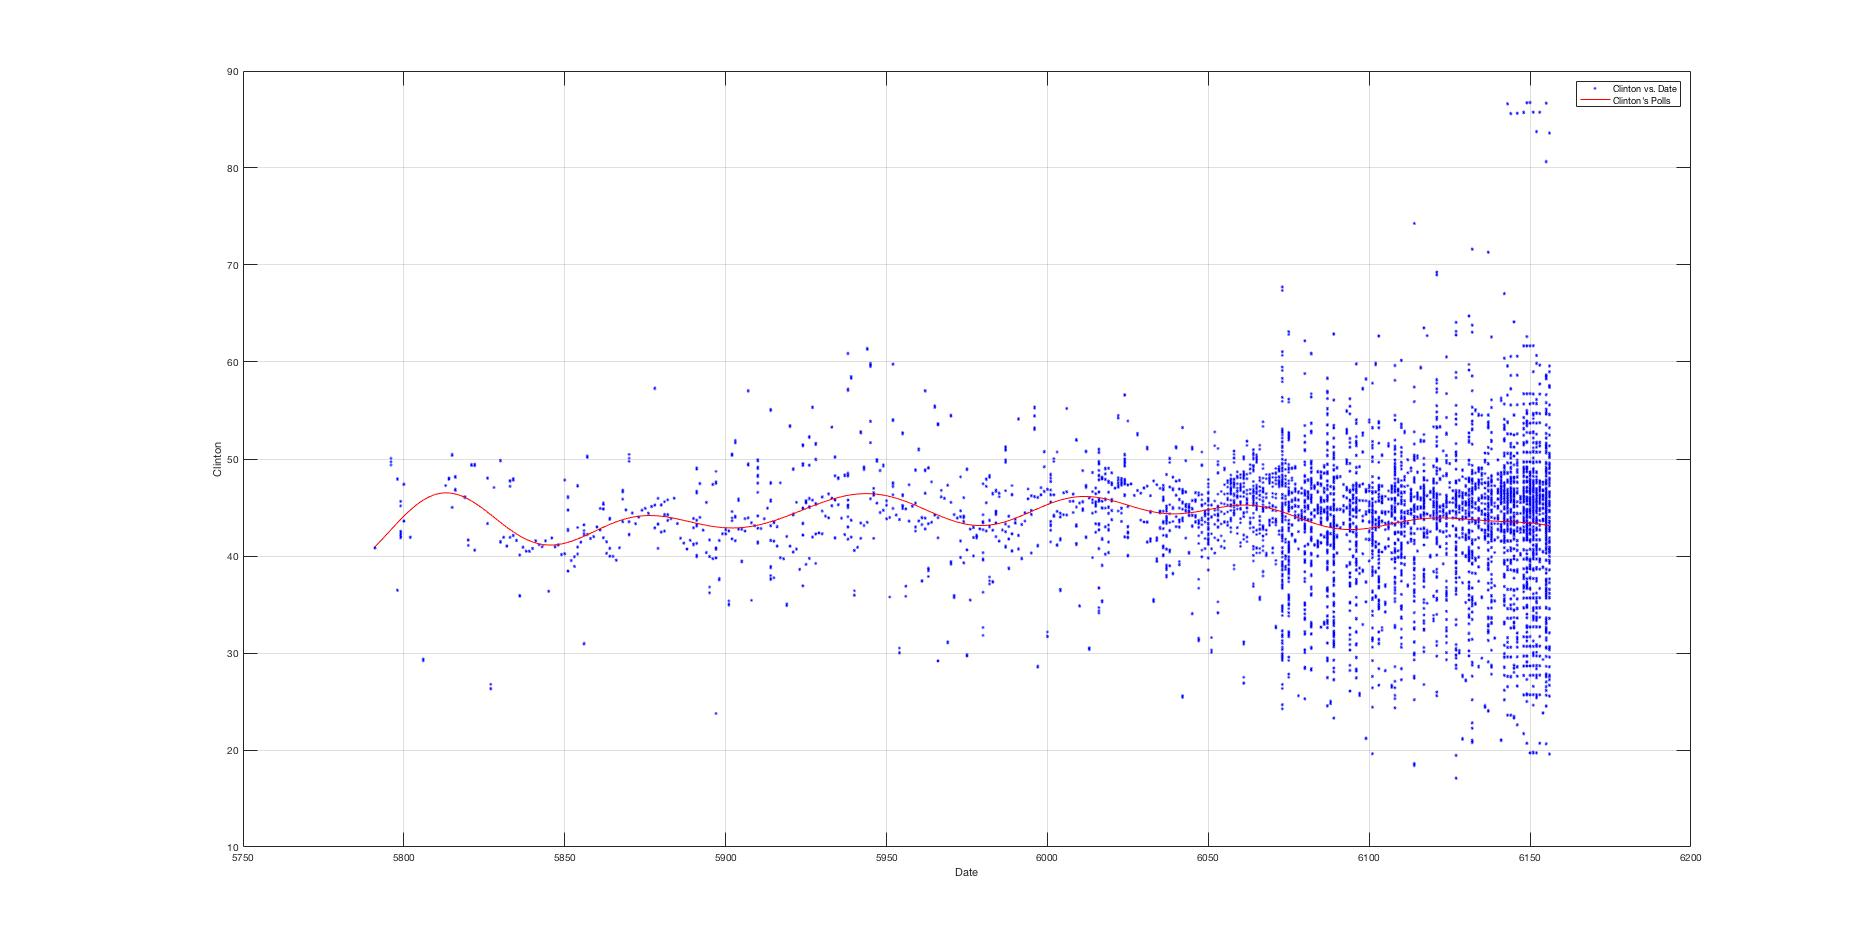
\includegraphics[width=\textwidth]{images/fourier/clinton.jpg}
    \caption{Clinton's Fourier Analysis}
\end{figure}
 \begin{figure}[H]
   \centering
     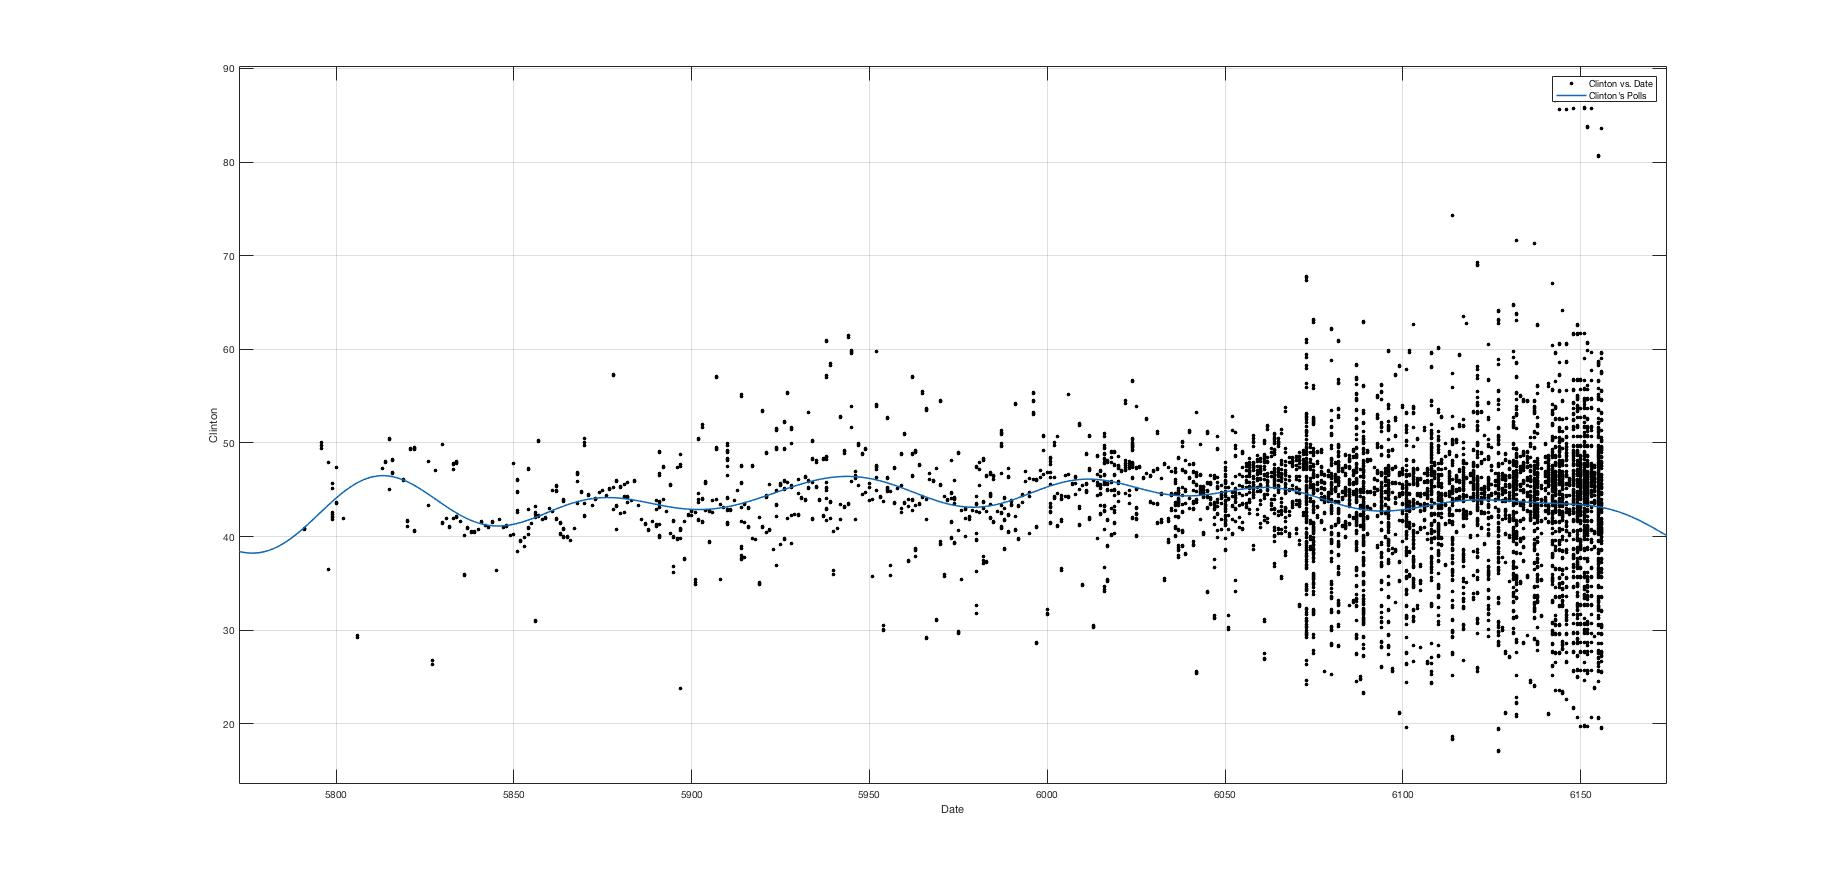
\includegraphics[width=\textwidth,height=6cm]{images/fourier/clintonlarge.jpg}
     \caption{Clintons's Fourier Extrapolation}
 \end{figure}
 \paragraph{Analysis} Clinton's Fourier analysis is very interesting. It actually shows her trending down towards the end, as was seen in the election.
  She doesn't trend below 50\%, but the trend down is very interesting to see. Her actual Fourier Analysis (of 8 terms) calculated by MATLAB with 95\% confidence is:
\newpage
\begin{gather*}
  f(x) =
           a_0 + a_1*cos(x*w) + b_1*sin(x*w) + \\
           a_2*cos(2*x*w) + b_2*sin(2*x*w) + a_3*cos(3*x*w) + b_3*sin(3*x*w) + \\
           a_4*cos(4*x*w) + b_4*sin(4*x*w) + a_5*cos(5*x*w) + b_5*sin(5*x*w) + \\
           a_6*cos(6*x*w) + b_6*sin(6*x*w) + a_7*cos(7*x*w) + b_7*sin(7*x*w) + \\
           a_8*cos(8*x*w) + b_8*sin(8*x*w)\\
\end{gather*}
Coefficients (with 95\% confidence bounds):
\begin{gather*}
   a_0 =       43.67 \\
   a_1 =       -1.41  \\
   b_1 =     -0.4745  \\
   a_2 =     -0.3162 \\
   b_2 =     0.06548  \\
   a_3 =     -0.4852  \\
   b_3 =      0.1476 \\
   a_4 =     -0.9232  \\
   b_4 =     -0.7231 \\
   a_5 =     -0.5835  \\
   b_5 =     -0.3198  \\
   a_6 =     -0.5982  \\
   b_6 =      -1.115  \\
   a_7 =      0.6509  \\
   b_7 =     -0.1644  \\
   a_8 =       0.402  \\
   b_8 =      -0.263  \\
   w =     0.01527  \\
\end{gather*}

\newpage
\subsection{Trump}
\begin{figure}[H]
  \centering
    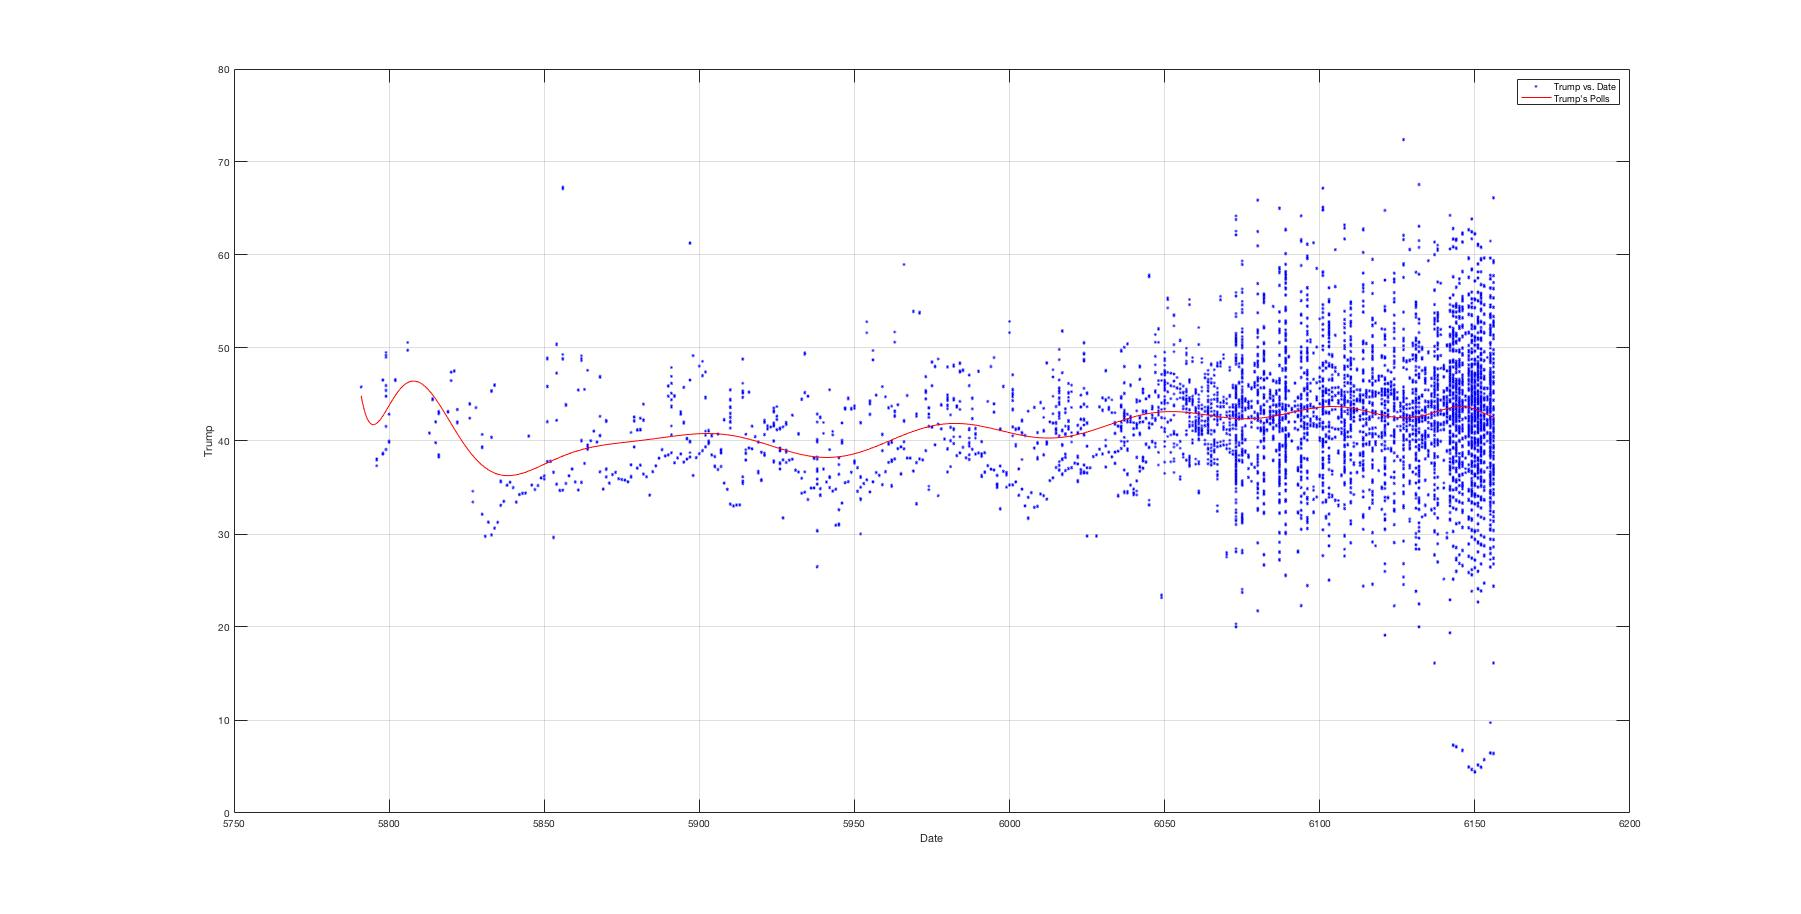
\includegraphics[width=\textwidth,height=6cm]{images/fourier/trump.jpg}
    \caption{Trump's Fourier Analysis}
\end{figure}
\begin{figure}[H]
  \centering
    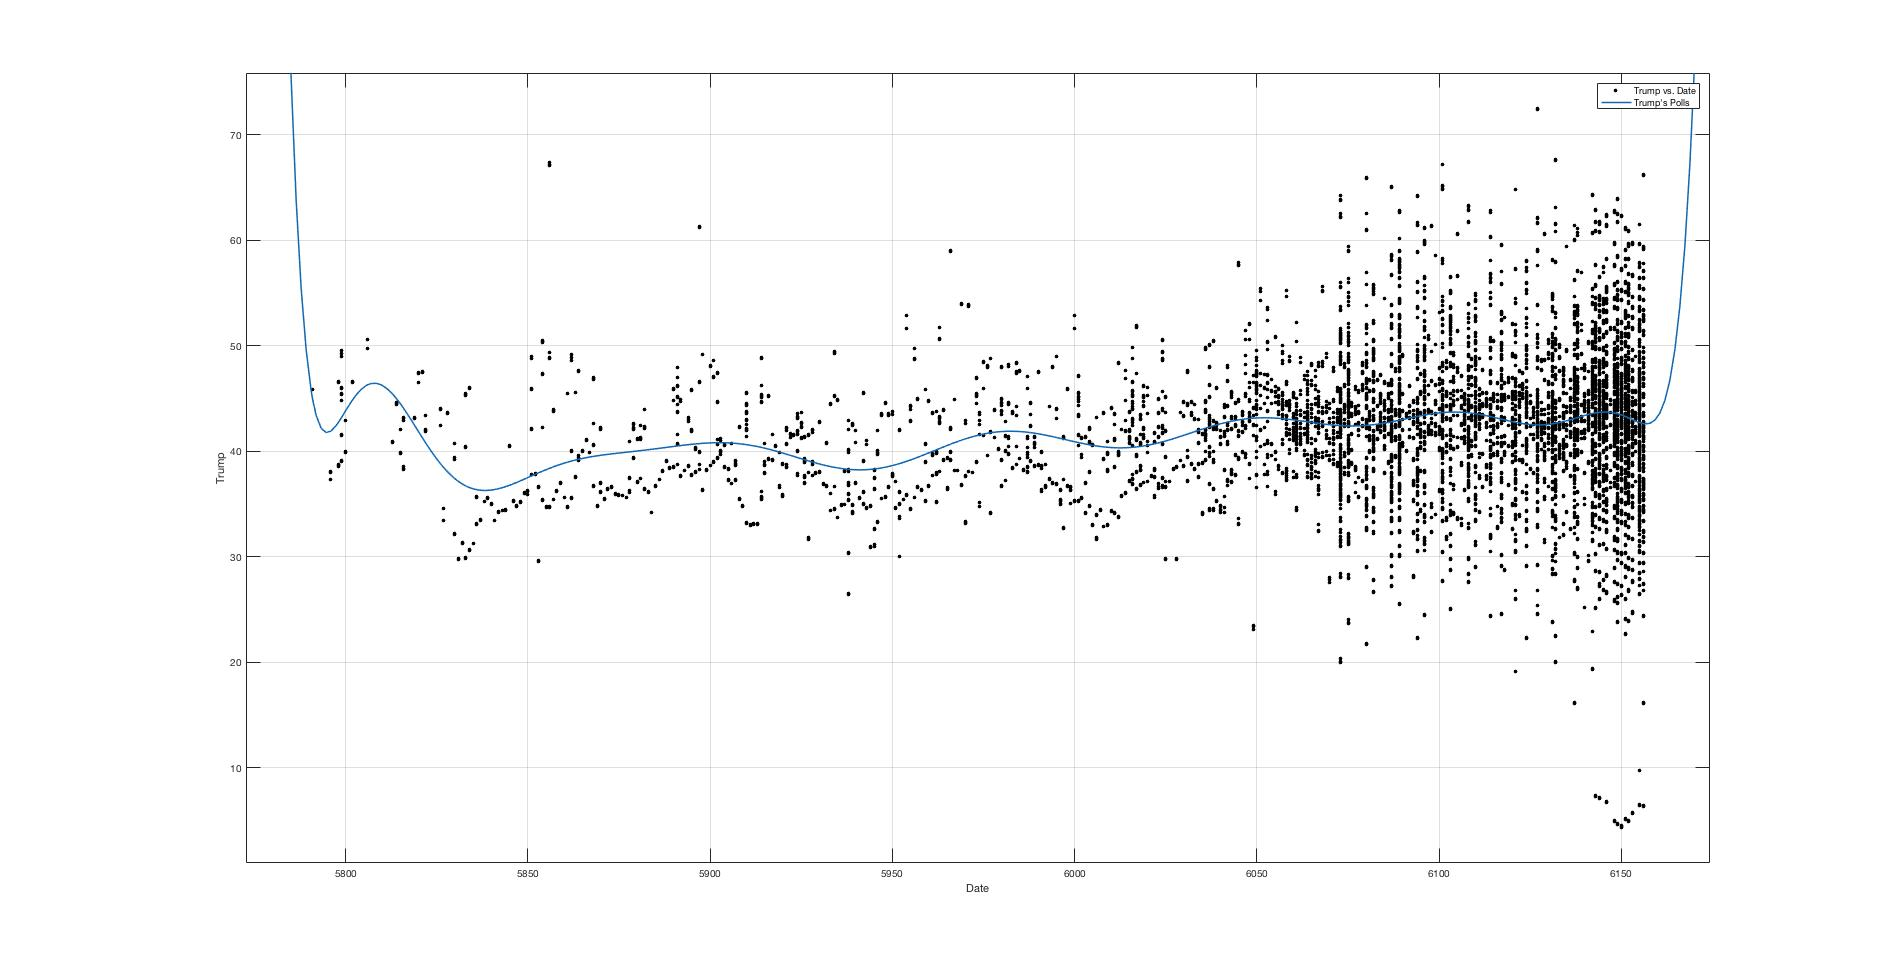
\includegraphics[width=\textwidth,height=6cm]{images/fourier/trumplarge.jpg}
    \caption{Trump's Fourier Extrapolation}
\end{figure}
\paragraph{Analysis} Trump's Fourier analysis is very interesting, too. We see the same trends as were reported by the polls, but based upon past history of Trump's numbers,
the Fourier function tells us that he will hit a point of inflection soon after November 8th. This is also apparent by the results of the election, but the point of inflection
was hit even sooner. Here's the actual analysis:
\newpage
\begin{gather*}
f(x) =
          a_0 + a_1*\cos(x*w) + b_1*\sin(x*w) +\\
          a_2*\cos(2*x*w) + b_2*\sin(2*x*w) + a_3*\cos(3*x*w) + b_3*\in(3*x*w) +\\
          a_4*\cos(4*x*w) + b_4*\sin(4*x*w) + a_5*\cos(5*x*w) + b_5*\sin(5*x*w) +\\
          a_6*\cos(6*x*w) + b_6*\sin(6*x*w) + a_7*\cos(7*x*w) + b_7*\sin(7*x*w) +\\
          a_8*\cos(8*x*w) + b_8*\sin(8*x*w)\\
\end{gather*}
Coefficients (with 95\% confidence bounds):
\begin{gather*}
  a_0 =   2.016e+06\\
  a_1 =    -1.9e+06  \\
  b_1 =   3.156e+06  \\
  a-2 =  -1.311e+06  \\
  b_2 =  -2.477e+06  \\
  a_3 =   1.756e+06  \\
  b_3 =    9.75e+04  \\
  a_4 =  -5.032e+05  \\
  b_4 =   7.383e+05  \\
  a_5 =  -1.482e+05  \\
  b_5 =  -3.238e+05  \\
  a_6 =   1.047e+05  \\
  b_6 =   1.206e+04  \\
  a_7 =  -1.273e+04  \\
  b_7 =   1.643e+04  \\
  a_8 =      -746.8  \\
  b_8 =       -1938  \\
  w =    0.007184 \\
\end{gather*}
\newpage
\section{Polls}
\section{Political Cartoons}
\newpage
\section{Wisconsin State Journal Endorsements}
\subsection{OUR ENDORSEMENT: Hillary Clinton. America must get this right.
}
\begin{enumerate}[*]
    \item She is disciplined, knowledgeable, and experienced
    \item Trump can’t even work with his own party
    \item Trump doesn’t have the support of Romney or McCain
    \item Clinton supported bipartisan bills
    \item 97-2 vote to confirm her as Secretary of State
    \item The far left views her as moderate, so party detractors shouldn’t be taken too seriously
\end{enumerate}
\subsection{Feingold More Likely to Get Things Done
}
\begin{enumerate}[*]
    \item Feingold helpd create the McCain-Feingold act
    \begin{enumerate}[-]
        \item Feingold banned gifts from lobbyists
    \end{enumerate}
    \item Feingold worked across the aisle
    \item Feingold knows Paul Ryan well
    \item Although Feingold has his faults, Johnson has no advantages.
    \item Feingold knows that climate change exists
\end{enumerate}
\subsection{Re-elect Paul Ryan and Mark Pocan to Congress
}
\begin{enumerate}[*]
    \item Pocan has gone out of his way to befriend republicans in congress
    \item Pocan has an engaging personality
    \item Pocan has a strong record of accomplishment
\end{enumerate}
\section{My Endorsements}
\subsection{Clinton, Feingold, and Pocan. Not for Party, but for Competence.}
The Republicans this year have not chosen the greatest candidates. Clinton has her flaws, but Trump is clearly unfit to be president. He has multiple laundry lists of faults and has shown that he will never have America’s interests at heart. Clinton is harassed by Republicans about Benghazi and her emails, which have both been investigated multiple times with no finding of wrongdoing. She is the clear choice because her opponent would be damaging. For Feingold, he could not push through an incredibly liberal agenda as Republicans would still be a strong force, but he would be an extra voice for climate change action, something that we need to enact immediately. Pocan is better than his opponent Theron because he has shown that he can work across the aisle and has a political personality, while Theron seems incapable of forming a logical argument.
\section{Election Results}
\section{Advice}



\end{document}
